\qquad A análise de complexidade do Quick Sort, considerando as
diferentes situações de entrada (crescente, decrescente e randômica),
foi realizada manuscrita, com a devida justificativa, escrevendo a
recorrência da função recursiva a partir do custo linear do
procedimento de partição e resolvendo-a para o melhor caso, o caso
médio e o pior caso, conforme exigido pelo enunciado do trabalho. A
contagem do número de execuções de cada linha da partição, com uma
constante de custo $c_i$ associada a cada linha, está detalhada no
resumo digitado que acompanha a figura.

\begin{figure}[htbp]
    \centering
    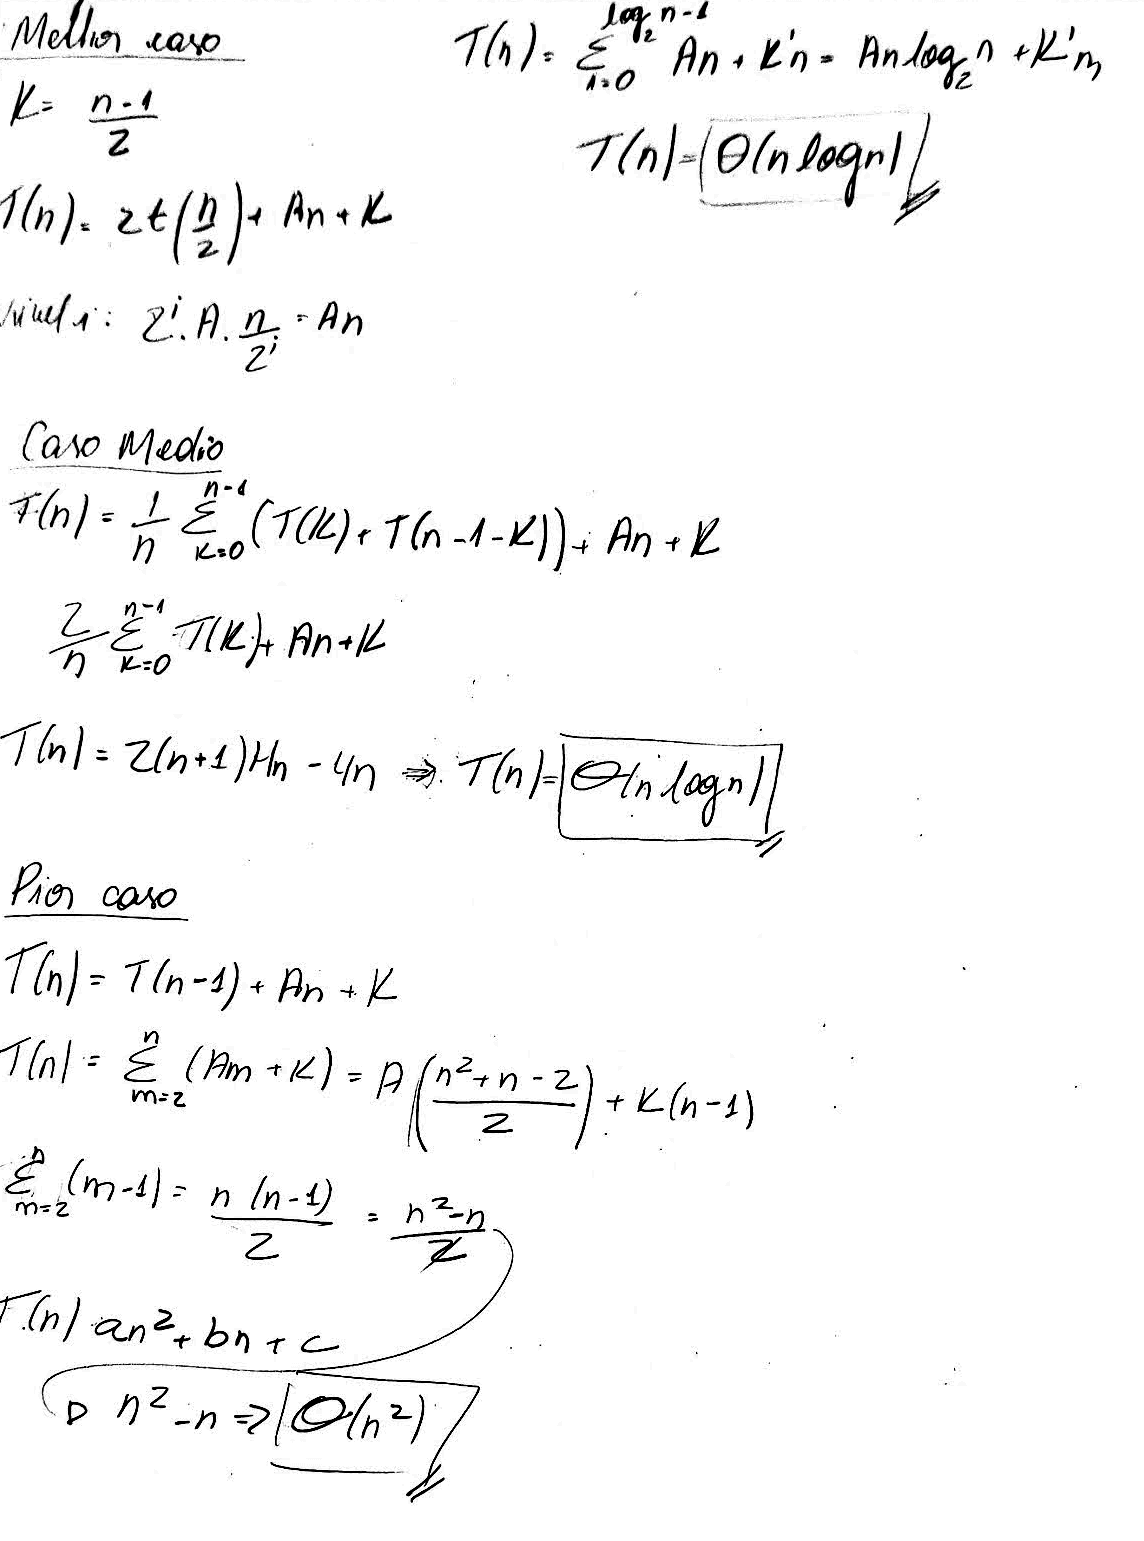
\includegraphics[width=14cm]{Imagens/Quick Sort/analise_complexidade.png}
    \caption{Análise de complexidade manuscrita do algoritmo Quick Sort}
    \label{fig:analise_complexidade_quick}
\end{figure}

\qquad Em resumo, a análise manuscrita chega às seguintes conclusões.

\qquad \textbf{Custo da partição.} Seja $m = fim - inicio + 1$ o número de
elementos do trecho e seja $k$ a quantidade de elementos do trecho
(sem contar o pivô) que são menores ou iguais ao pivô, de modo que
$0 \le k \le m-1$. Somando as execuções de cada linha de
\texttt{ParticionaVersao1}, obtém-se
\[
T_P(m) = c_2\,m + c_3\,(m-1) + c_4\,k + (c_1+c_5+c_6),
\]
Escrevendo essa expressão na forma $T_P(m) = A\,m + K$ --- notação
usada na figura ---, tem-se $c_2+c_3 \le A \le c_2+c_3+c_4$, pois
$0 \le k \le m-1$: na entrada crescente ($k = 0$) vale
$A = c_2+c_3$ e na decrescente ($k = m-1$) vale $A = c_2+c_3+c_4$.
Ainda de $0 \le k \le m-1$, vale
\[
c_2\,m + c_3\,(m-1) + K \;\le\; T_P(m) \;\le\; (c_2+c_3+c_4)\,m - (c_3+c_4) + K ,
\]
com $K = c_1+c_5+c_6$ constante. As duas cotas são funções lineares em
$m$, logo $T_P(m) = \Theta(m)$: a partição \textbf{tem tempo linear},
qualquer que seja a ordem dos dados, porque cada elemento do trecho é
visitado exatamente uma vez pelo laço (o índice $j$ avança de
$inicio+1$ até $fim$ e nunca retrocede), realizando um número
constante de operações por elemento. São feitas exatamente $m-1$
comparações e, no máximo, $m$ trocas.

\qquad \textbf{Recorrência.} Se o pivô termina na posição $p$, o trecho
de $m$ elementos se divide em um trecho de $k = p - inicio$ elementos
à esquerda e um de $m - 1 - k$ à direita, e o próprio pivô não entra
em nenhuma chamada seguinte. Logo
\[
T(n) = T(k) + T(n-1-k) + T_P(n) = T(k) + T(n-1-k) + \Theta(n),
\]
com $T(1) = T(0) = \Theta(1)$. Ao contrário do Merge Sort, em que a
divisão é sempre exatamente ao meio, aqui o valor de $k$ depende dos
dados --- e é justamente isso que separa os três casos.

\qquad \textbf{Melhor caso ($k = \lfloor (n-1)/2 \rfloor$):} o pivô é a
mediana do trecho e as duas partições ficam do mesmo tamanho. A
recorrência torna-se $T(n) = 2\,T(n/2) + \Theta(n)$, idêntica à do
Merge Sort: a árvore de recursão tem $\log_2 n$ níveis e cada nível
custa $\Theta(n)$, de modo que
$T(n) = \Theta(n \log n)$ --- resultado que também decorre do caso 2
do Teorema Mestre (CORMEN et al., 2009), com $a = 2$, $b = 2$ e
$f(n) = \Theta(n)$. O número de comparações é cerca de
$n \log_2 n$.

\qquad \textbf{Pior caso ($k = 0$ ou $k = n-1$):} o pivô é o menor ou o
maior elemento do trecho, uma das partições fica vazia e a outra com
$n-1$ elementos. A recorrência degenera para
$T(n) = T(n-1) + \Theta(n)$, cuja solução é
\[
T(n) = \sum_{m=2}^{n} \Theta(m) = \Theta\!\left(\frac{n(n+1)}{2} - 1\right) = \Theta(n^2),
\]
com exatamente
$\sum_{m=2}^{n} (m-1) = \dfrac{n(n-1)}{2}$ comparações. Para a
\textbf{versão 1}, em que o pivô é o primeiro elemento, esse pior caso
ocorre exatamente nas entradas \textbf{crescente} ($k = 0$ em todas as
partições, porque o primeiro elemento é sempre o menor) e
\textbf{decrescente} ($k = n-1$, porque o primeiro elemento é sempre o
maior) --- isto é, nas duas entradas ordenadas exigidas pelo trabalho,
e não em uma entrada artificial. É um resultado que contraria a
intuição: para a versão 1 do Quick Sort, dados já ordenados são o
cenário mais desfavorável, e não o mais favorável.

\qquad \textbf{Caso médio (entrada randômica):} supondo que o pivô tenha
a mesma probabilidade de terminar em qualquer uma das $n$ posições,
\[
T(n) = \frac{1}{n}\sum_{k=0}^{n-1}\big[T(k) + T(n-1-k)\big] + \Theta(n),
\]
cuja solução é $T(n) \approx 2(n+1)H_n - 4n \approx 1{,}386\,n\log_2 n$,
onde $H_n$ é o $n$-ésimo número harmônico; portanto
$T(n) = \Theta(n \log n)$, apenas cerca de 39\% acima do melhor caso
(CORMEN et al., 2009). Ou seja, o caso médio do Quick Sort tem a mesma
ordem de grandeza do melhor caso, e é por isso que, apesar do pior
caso quadrático, o algoritmo é considerado o mais rápido na prática
para entradas sem ordenação prévia.

\qquad \textbf{A versão 2 (pivô igual à média).} A média aritmética do
trecho é sempre um valor entre o menor e o maior elemento, logo nunca
produz uma partição vazia: isso elimina o pior caso da versão 1 nas
entradas ordenadas. Em uma entrada crescente ou decrescente, a média
cai exatamente no meio do trecho, as partições ficam equilibradas e o
algoritmo atinge o seu \textbf{melhor caso}, $\Theta(n \log n)$. O
cálculo da média percorre o trecho uma segunda vez, somando mais
$\Theta(m)$ ao custo da partição, o que dobra a constante mas não
altera a ordem de complexidade. Em teoria a versão 2 também tem pior
caso $\Theta(n^2)$ --- bastaria uma distribuição em que a média
ficasse sistematicamente próxima de um dos extremos do trecho, como
valores que crescem exponencialmente ---, mas nenhuma das três
entradas exigidas pelo trabalho produz esse comportamento.

\qquad \textbf{Memória e estabilidade.} As duas versões ordenam
\textit{no próprio vetor} (ordenação \textit{in place}), sem vetor
auxiliar, ao contrário do Merge Sort, que precisa de $\Theta(n)$ de
memória adicional. A memória extra usada é apenas a da pilha de
recursão. Nenhuma das duas versões é \textbf{estável}: as trocas da
partição podem inverter a ordem relativa de elementos iguais.

\qquad \textbf{Verificação experimental das contagens.} Para conferir
essas previsões foi executada uma versão do algoritmo instrumentada
para contar as operações (usada apenas para esta verificação, fora do
código entregue). Os números confirmam a análise:

\begin{itemize}
    \item \textbf{Versão 1, entradas crescente e decrescente:} foram
    contadas exatamente 499.500 comparações para $n = 1.000$ e
    49.995.000 para $n = 10.000$, valores que coincidem com a fórmula
    do pior caso $n(n-1)/2$ --- confirmando que as duas entradas
    ordenadas são, de fato, o pior caso. Para $n = 1.000.000$ a mesma
    fórmula prevê 499.999.500.000 comparações, cerca de meio trilhão;
    \item \textbf{Versão 1, entrada randômica:} 24.149.675 comparações
    para $n = 1.000.000$, próximo das 24.785.500 previstas por
    $2(n+1)H_n - 4n$ (diferença de 2,6\%) e \textbf{vinte mil vezes}
    menos que no pior caso;
    \item \textbf{Versão 2:} 19.000.019 comparações na entrada
    crescente e 19.000.036 na decrescente, para $n = 1.000.000$,
    próximas de $n \log_2 n \approx 19.931.569$, com profundidade
    máxima de recursão igual a 20 ($\lceil \log_2 10^6 \rceil = 20$) e
    partições perfeitamente equilibradas --- ou seja, o melhor caso,
    como previsto. Na entrada randômica foram 21.334.769 comparações;
    \item \textbf{Profundidade da recursão:} medida sobre a versão
    puramente recursiva (sem a eliminação da recursão de cauda
    descrita na seção anterior), a profundidade atingiu exatamente
    50.000 níveis para $n = 50.000$ nas entradas crescente e
    decrescente, contra apenas 40 níveis na entrada randômica. Isso
    confirma que, sem essa medida, o pior caso com 1.000.000 de
    elementos esgotaria a pilha do programa; com ela, a profundidade
    observada foi de 2 níveis nas entradas ordenadas e 14 níveis na
    randômica.
\end{itemize}

\qquad Os resultados experimentais apresentados na próxima seção deste
capítulo são compatíveis com essa análise: a versão 1 cresceu de forma
claramente quadrática nas duas entradas ordenadas e de forma
$n \log n$ na entrada randômica, enquanto a versão 2 cresceu de forma
$n \log n$ nas três situações.
